\documentclass[a4paper,12pt]{article}

\usepackage[ngerman]{babel}
\usepackage[utf8]{inputenc}
\usepackage[T1]{fontenc}
\usepackage{marvosym}
\usepackage{array}
\usepackage{amsmath}
\usepackage{mathrsfs,amssymb}
\usepackage{ifthen,calc}
\usepackage{theorem}
\usepackage{graphicx}
\usepackage[left=2cm,right=2cm,top=1.5cm,bottom=2cm]{geometry}
\usepackage{enumerate}
\usepackage{tabularx} % automatische Spaltenbreite
\usepackage{booktabs}
 \usepackage[T1]{fontenc}
\usepackage[utf8]{inputenc}
\usepackage{stmaryrd}
\usepackage{setspace}
\usepackage{mathrsfs}
\usepackage[ngerman]{babel}
\usepackage{amssymb}
\usepackage{amsmath}
\usepackage{enumitem}
\usepackage[colorlinks,linkcolor=black]{hyperref} 
\usepackage{fancyhdr}
\usepackage{subcaption}
\usepackage{graphicx}
\usepackage{lipsum}
\usepackage{float}
\usepackage{color}
\usepackage{listings}


\usepackage{listings}
\usepackage{color}
\usepackage{hyperref}
\usepackage{longtable}
\hypersetup{
     colorlinks   = true,
     citecolor    = gray,
     linkcolor    = blue,
     urlcolor     = blue,
}

\definecolor{mygreen}{rgb}{0,0.6,0}
\definecolor{mygray}{rgb}{0.5,0.5,0.5}
\definecolor{mymauve}{rgb}{0.58,0,0.82}

\lstset{ %
  backgroundcolor=\color{white},   % choose the background color; you must add \usepackage{color} or \usepackage{xcolor}
  basicstyle=\small,        % the size of the fonts that are used for the code
  breakatwhitespace=false,         % sets if automatic breaks should only happen at whitespace
  breaklines=true,                 % sets automatic line breaking
  captionpos=b,                    % sets the caption-position to bottom
  commentstyle=\color{mygreen},    % comment style
  deletekeywords={...},            % if you want to delete keywords from the given language
  escapeinside={\%*}{*)},          % if you want to add LaTeX within your code
  extendedchars=true,              % lets you use non-ASCII characters; for 8-bits encodings only, does not work with UTF-8
  frame=single,	                   % adds a frame around the code
  keepspaces=true,                 % keeps spaces in text, useful for keeping indentation of code (possibly needs columns=flexible)
  keywordstyle=\color{blue},       % keyword style
  language=VHDL,                 % the language of the code
  otherkeywords={*,...},           % if you want to add more keywords to the set
  numbers=left,                    % where to put the line-numbers; possible values are (none, left, right)
  numbersep=5pt,                   % how far the line-numbers are from the code
  numberstyle=\tiny\color{mygray}, % the style that is used for the line-numbers
  rulecolor=\color{black},         % if not set, the frame-color may be changed on line-breaks within not-black text (e.g. comments (green here))
  showspaces=false,                % show spaces everywhere adding particular underscores; it overrides 'showstringspaces'
  showstringspaces=false,          % underline spaces within strings only
  showtabs=false,                  % show tabs within strings adding particular underscores
  stepnumber=1,                    % the step between two line-numbers. If it's 1, each line will be numbered
  stringstyle=\color{mymauve},     % string literal style
  tabsize=2,	                   % sets default tabsize to 2 spaces
  linewidth=15cm,
  title=\lstname                   % show the filename of files included with \lstinputlisting; also try caption instead of title
}

\usepackage{caption}
\captionsetup[lstlisting]{font={scriptsize}}
\DeclareGraphicsExtensions{.pdf,.png,.jpg}

\pagestyle{fancy}
\lfoot{Carl Schaffer}
\rfoot{carl.schaffer@cern.ch}
\cfoot{-\thepage-}
\renewcommand{\headrulewidth}{0.6pt}
\renewcommand{\footrulewidth}{0.6pt}
\setlength{\headheight}{37pt}
\setlength{\parindent}{0pt}
\renewcommand{\familydefault}{\sfdefault}

\newcommand{\exercise}[2]{\section{#1}\hfill{}\\}

\newcommand{\doublefig}[2]{\begin{center}
  \begin{tabular}{ll}
    a.) &b.)\\
    \includegraphics[width=.3\textwidth]{#1}&  \includegraphics[width=.3\textwidth]{#2} 
  \end{tabular}
\end{center}
}

\newcommand{\doublefignolabel}[2]{\begin{center}
  \begin{tabular}{ll}
    \includegraphics[width=.2\textwidth]{#1}&\includegraphics[width=.3\textwidth]{#2}
  \end{tabular}
\end{center}
}


\newcommand{\signal}[1]{\texttt{#1}}
\newcommand{\stdl}{\lstinline$standard_logic$}
\newcommand{\stdlv}[2]{\lstinline$standard_logic_vector(#1 downto #2)$}
\newcommand{\vhdl}[1]{\lstinline$#1$}
\newcommand{\loghi}{\vhdl{'1'}}
\newcommand{\loglo}{\vhdl{'0'}}

\newcommand*{\bashcode}{\lstinline[{language=[LaTeX]TeX}]}
\newcommand{\bash}[1]{\bashcode$#1$}
\newcommand{\git}{\texttt{GIT}}

\newcommand{\nandGate}{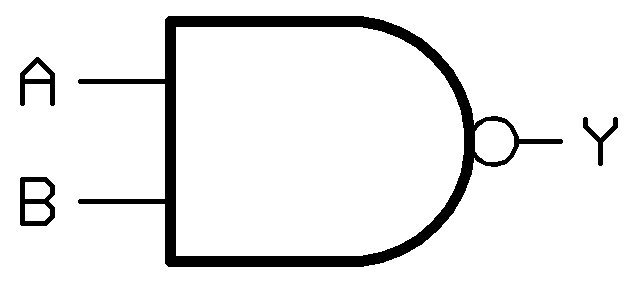
\includegraphics[width=3cm]{./images/nand}}
\newcommand{\andGate}{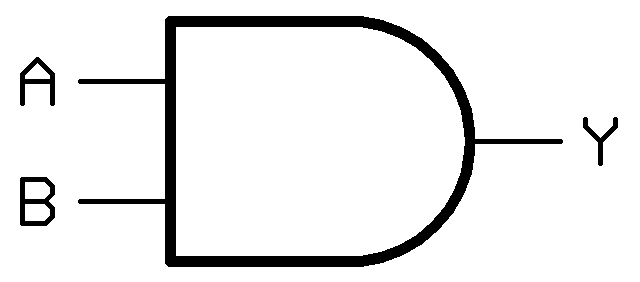
\includegraphics[width=3cm]{./images/and}}
\newcommand{\notGate}{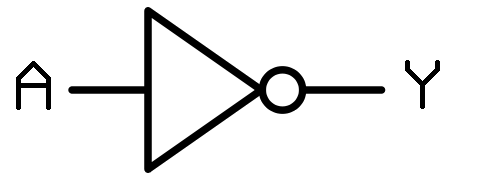
\includegraphics[width=3cm]{./images/not}}
\newcommand{\xorGate}{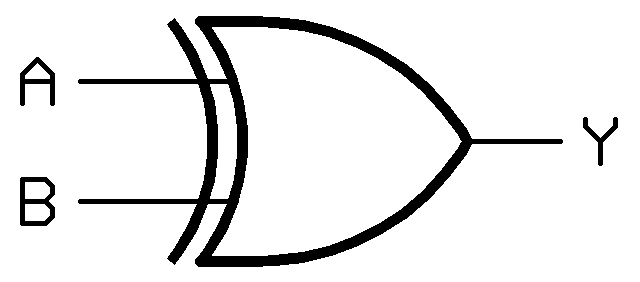
\includegraphics[width=3cm]{./images/xor}}
\newcommand{\orGate}{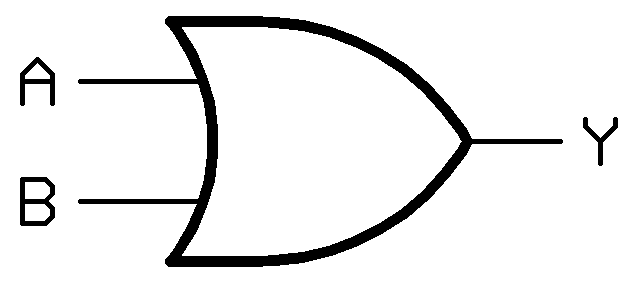
\includegraphics[width=3cm]{./images/or}}

\newcommand{\ise}{XILINX ISE}

\newcommand{\al}[1]{
\begin{align}
#1
\end{align}
}


\newcommand{\pic}[2]{\begin{center}\includegraphics[width=#1\linewidth]{#2}\end{center}}

\newcommand{\nn}{\nonumber}

\newcommand{\lr}[1]{
\left( #1 \right)
}

\newcommand{\head}[3]{%
\pagestyle{empty}

\vspace{-1.5cm}
\noindent Albert-Ludwigs-Universität Freiburg \hfill SS #1\\
\hrule

\begin{center}
  \section*{Übungsblatt #2}
  \large zur Vorlesung \textit{Einführung in die moderne Digitalelektronik} \normalsize \\
  \vspace{0.5cm}
  Prof. Dr. Horst Fischer, #3\\
\end{center}
\hrule
\vspace{0.5cm}
}



%%%%%% dokument %%%%%%%%%%%%%%%%%%%%%%%%%%%%%%%%%%%%%%%%%
\begin{document}
\head{2021}{2}{Daniel Baur}


\newboolean{showsolution}
\setboolean{showsolution}{false}




%%%%%%%%%%%%%%%%%%%%%%%%%%%%%%%%%%% 1 LOGIKGATTER %%%%%%%%%%%%%%%%%%%%%%%%%%%%%%%%%%%%%%%%%%%%%%%%%%%
\part*{Boolsche Algebra}


\ifthenelse{\boolean{showsolution}}{
\exercise{Logikgatter}{3}
Vervollständigen sie die Wahrheitstabellen , geben sie die
entsprechende Bool'sche Gleichung an und benennen sie das dargestellte
Gatter:
\section*{Lösung}
\begin{center}
  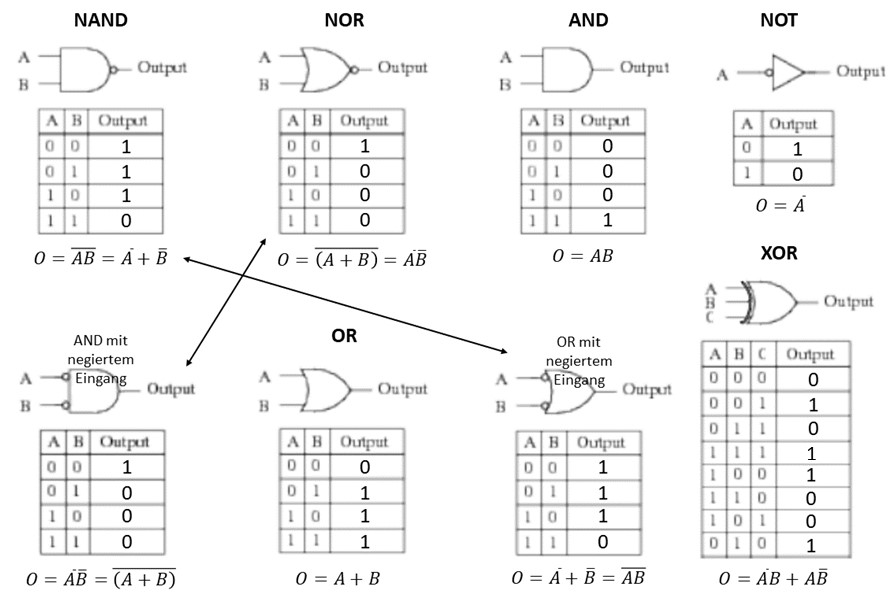
\includegraphics[width = 0.99\textwidth{}]{./images/Blatt1_Aufgabe1_Bild1_crop_crop.jpg}
\end{center}
}{
\exercise{Logikgatter}{3}
Vervollständigen sie die Wahrheitstabellen , geben sie die
entsprechende Bool'sche Gleichung an und benennen sie das dargestellte
Gatter:
\begin{center}
  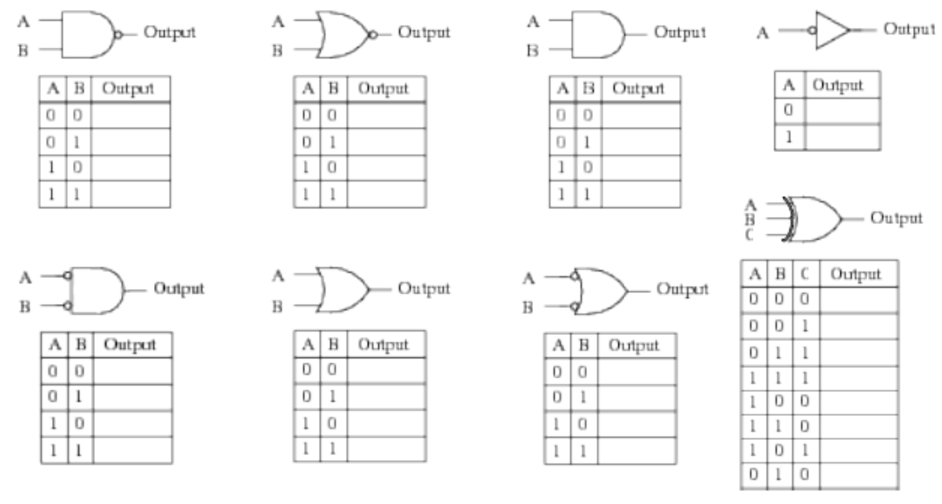
\includegraphics[width = 0.7\textwidth{}]{./images/02776x01.pdf}
\end{center}
}










%%%%%%%%%%%%%%%%%%%%%%%%%%%%%%%%%%% 2 VERKETTUNG VON GATTERN %%%%%%%%%%%%%%%%%%%%%%%%%%%%%%%%%%%%%%%%%%%%%%%%%%%
\ifthenelse{\boolean{showsolution}}{
\clearpage
}{}


% \newpage{}

\exercise{Verkettung von Gattern}{2}

% \subsection{Verkettungen von Gattern}
\label{sec:gl}
Geben sie Gleichungen für die Signale an den markierten Stellen an:


\begin{center}
  \begin{tabular}{ll}
    a.) &b.)\\
    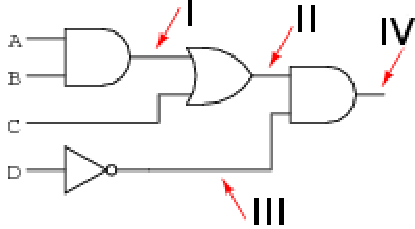
\includegraphics[width=.3\textwidth]{./images/01301x01_commented.pdf}&  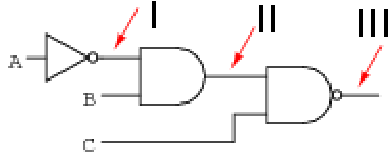
\includegraphics[width=.3\textwidth]{./images/02783x01.pdf} 
  \end{tabular}

  % \begin{center}
\end{center}

\ifthenelse{\boolean{showsolution}}{
\section*{Lösung}
\begin{enumerate}
\item[a.)]
\al{
\text{I} &= A\cdot B \nn \\
\text{II} &= \lr{A\cdot B} + C \nn \\
\text{III} &= \overline{D} \nn \\
\text{IV} &= \left[\lr{A\cdot B} + C\right] \cdot \overline{D} \nn 
}
\item[b.)]
\al{
\text{I} &= \overline{A} \nn \\
\text{II} &= \overline{A} \cdot B \nn \\
\text{III} &= \overline{\overline{A} \cdot B\cdot C} \nn
}
\end{enumerate}
}{}




%%%%%%%%%%%%%%%%%%%%%%%%%%%%%%%%%%% 3 BOOLSCHE ALGEBRA: GLEICHUNGEN %%%%%%%%%%%%%%%%%%%%%%%%%%%%%%%%%%%%%%%%%%%%%%%%%%%
\ifthenelse{\boolean{showsolution}}{
\clearpage
}{}



\exercise{Bool'sche Algebra: Gleichungen}{3} Vereinfachen sie folgende
Ausdrücke mit Hilfe der Rechenregeln für Bool'sche Algebra:

\begin{enumerate}[label=\alph*.)]
\item[a.)] $F=\overline{A}BC+CD+\overline{A}+\overline{C}$
\item[b.)*]
  $F=\overline{A}~\overline{B}+\overline{A}B\overline{C}+\overline{A+\overline{C}}$
\end{enumerate}

\ifthenelse{\boolean{showsolution}}{
\section*{Lösung}
\begin{enumerate}
\item[a.)]
\begin{align*}
F &= \overline{A}BC+CD+\overline{A}+\overline{C} & \text{(Kommutativgesetz)} \nn \\
 &= \overline{A}BC +\overline{A} +CD +\overline{C} & \text{(Absorptionsgesetz)}  \nn \\
 &= \overline{A} +CD +\overline{C}  & \text{(Absorptionsgesetz)}  \nn \\
 &= \overline{A} +CD +\overline{C} +\overline{C}D  & \text{(Kommutativgesetz)}  \nn \\
&= \overline{A} +\overline{C} +CD +\overline{C}D  & \text{(Distributivgesetz)}  \nn \\
&= \overline{A} +\overline{C} +D(C +\overline{C})  & \text{(Existenz v. Inversen bzgl. $+$)}  \nn \\
 &= \overline{A} +\overline{C} +D \nn
\end{align*}
\textbf{Absorptionsgesetz}:\\
Seien $A,B\in\{0,1\}$ beliebig. Dann gilt:
\al{
A = A\cdot 1 = A\cdot (B+1) = (A\cdot B) + (A\cdot 1) =  AB + A \nn
}
\item[b.)]
\begin{align*}
F &= \overline{A}~\overline{B}+\overline{A}B\overline{C}+\overline{A+\overline{C}}  & \text{(De Morgansche Gesetze)} \nn \\
 &= \overline{A}~\overline{B}+\overline{A}B\overline{C}+\overline{A}C  & \text{(Distributivgesetz)} \nn \\
 &= \overline{A}\lr{\overline{B} +B\overline{C} +C}  & \text{(Absorptionsgesetz)} \nn \\
 &= \overline{A}\lr{\overline{B} +B\overline{C} +C + CB}  & \text{(Distributivgesetz)} \nn \\
 %&= \overline{A}\lr{\overline{B} +B\underbrace{\lr{\overline{C} + C}}_{=1} +C} & \text{(Existenz v. Inversen)}  \nn \\
 &= \overline{A}\lr{\overline{B} +B\lr{\overline{C} + C} +C} & \text{(Existenz v. Inversen bzgl. $+$)}  \nn \\
 %&= \overline{A}\lr{\underbrace{\overline{B} +B}_{=1} +C}  & \text{(Existenz v. Inversen)} \nn \\
 &= \overline{A}\lr{\overline{B} +B +C}  & \text{(Assoziativgesetz)} \nn \\
 &= \overline{A}\lr{(\overline{B} +B) +C}  & \text{(Existenz v. Inversen bzgl. $+$)} \nn \\
 %&= \overline{A}\underbrace{\lr{1 +C}}_{=1} & \text{(Addition mit $1$)}  \nn \\
 &= \overline{A}\lr{1 +C} & \text{(Addition mit $1$)}  \nn \\
 &= \overline{A} \nn
\end{align*}
\end{enumerate}

}{}







%%%%%%%%%%%%%%%%%%%%%%%%%%%%%%%%%%% 4 BOOLSCHE ALGEBRA: KOMPLEMENT %%%%%%%%%%%%%%%%%%%%%%%%%%%%%%%%%%%%%%%%%%%%%%%%%%%
\ifthenelse{\boolean{showsolution}}{
\clearpage
}{}


\exercise{Bool'sche Algebra: Komplement}{4} Bilden sie das Komplement der
folgenden Ausdrücke und vereinfachen sie:
\begin{enumerate}[label=\alph*.)]
\item[a.)] $F=A+B(CD)$
\item[b.)*]
  $F=A\overline{B}C+(\overline{A}+B+D)(AB\overline{D}+\overline{B})$
\end{enumerate}
 
\ifthenelse{\boolean{showsolution}}{
\section*{Lösung}
\begin{enumerate}
\item[a.)]
\begin{align*}
\overline{F} &= \overline{A+B(CD)}  & \text{(De Morgansche Gesetze)}   \nn \\
 &= \overline{A}\cdot\overline{B(CD)} & \text{(De Morgansche Gesetze)}  \nn \\
 &= \overline{A}\cdot\lr{\overline{B}+\overline{CD}}  & \text{(De Morgansche Gesetze)} \nn \\
 &= \overline{A}\cdot\lr{\overline{B} + \overline{C} + \overline{D}} \nn
\end{align*}
\item[b.)]
\begin{align*}
\overline{F} &= \overline{A\overline{B}C+(\overline{A}+B+D)(AB\overline{D}+\overline{B})} & \text{(De Morgansche Gesetze)}  \nn \\
 &=  \overline{A\overline{B}C} \cdot \overline{(\overline{A}+B+D)(AB\overline{D}+\overline{B})} & \text{(De Morgansche Gesetze)} \nn \\
 &=  \lr{\overline{A} +B +\overline{C}} \cdot \lr{\overline{(\overline{A}+B+D)} +\overline{(AB\overline{D}+\overline{B})}}  & \text{(De Morgansche Gesetze)}\nn \\
 &=  \lr{\overline{A} +B +\overline{C}} \cdot \lr{A\overline{B}~\overline{D} +\lr{\overline{AB\overline{D}}\cdot B}} & \text{(De Morgansche Gesetze)} \nn \\
 &=  \lr{\overline{A} +B +\overline{C}} \cdot \lr{A\overline{B}~\overline{D} +\lr{\lr{\overline{A} +\overline{B} +D}\cdot B}} & \text{(Distributivgesetz)} \nn \\
 &=  \lr{\overline{A} +B +\overline{C}} \cdot \lr{A\overline{B}~\overline{D} +\overline{A}B +\overline{B}B +BD} & \text{(Existenz v. Inversen bzgl. $\cdot$)} \nn \\
 &=  \lr{\overline{A} +B +\overline{C}} \cdot \lr{A\overline{B}~\overline{D} +\overline{A}B +BD} & \text{(Distributivgesetz)} \nn \\
 &=\,\,\,\, \overline{A}A\overline{B}~\overline{D} +\overline{A}~\overline{A}B +\overline{A}BD & \text{(Existenz v. Inversen bzgl. $\cdot$)} \nn \\
 &\quad+A\overline{B}B\overline{D} +\overline{A}BB +BBD \nn \\
 &\quad+A\overline{B}~\overline{C}~\overline{D} +\overline{A}B\overline{C} +B\overline{C}D \nn \\
 &=\,\,\,\, \overline{A}~\overline{A}B +\overline{A}BD & \text{(Duplikate)} \nn \\
 &\quad +\overline{A}BB +BBD \nn \\
 &\quad+A\overline{B}~\overline{C}~\overline{D} +\overline{A}B\overline{C} +B\overline{C}D \nn \\
 &=\,\,\,\, \overline{A}B +\overline{A}BD & \text{(Absorptionsgesetz)} \nn \\
 &\quad  +BD \nn \\
 &\quad+A\overline{B}~\overline{C}~\overline{D}  +B\overline{C}D \nn \\
  &= \overline{A}B +BD +A\overline{B}~\overline{C}~\overline{D} \nn
\end{align*}
\end{enumerate}

}{}




% Schreibweise: $AB \equiv A\cdot B$


%%%%%%%%%%%%%%%%%%%%%%%%%%%%%%%%%%% 5 RECHNEN MIT BINÄRZAHLEN %%%%%%%%%%%%%%%%%%%%%%%%%%%%%%%%%%%%%%%%%%%%%%%%%%%
\ifthenelse{\boolean{showsolution}}{
\clearpage
}{}


\exercise{Rechnen mit Binärzahlen}{4} Bei der Programmierung in VHDL
ist es wichtig mit dem Binärsystem vertraut zu sein. Zahlen werden als
Abfolgen der Ziffern '\texttt{0}' und '\texttt{1}' dargestellt. Jede
Ziffer stellt (von rechts nach links aufsteigend) eine entsprechende
Zweierpotenz dar:

\begin{center}
  \begin{tabular}{|c|c|c|c|c|}
    \hline{}
    $2^4$&$2^3$&$2^2$&$2^1$&$2^0$\\
    \hline{}
    16&8&4&2&1\\\hline
  \end{tabular}
\end{center}

Die Binärzahl \texttt{10101} entspricht also
$(16\cdot 1)+(8\cdot 0)+(4\cdot 1)+(2\cdot 0)+(1\cdot 1)=21$ im
Zehnersystem. Berechnen sie:


\noindent\parbox[t]{2.4in}{\raggedright%

\begin{enumerate}[label=\alph*.)]
\item[a.)] $\texttt{101}+\texttt{1011}$
\item[b.)] $\texttt{111}+\texttt{0001}$
\item[c.)] $\texttt{1000}+\texttt{0011}$
\item[d.)] $\texttt{1101}+\texttt{1011}$
\end{enumerate}
}%
\parbox[t]{2.4in}{\raggedright%

\begin{enumerate}[label=\alph*.)]
\setcounter{enumi}{4}
\item[e.)*] $\texttt{1101}-\texttt{11}$
\item[f.)*] $\texttt{1000}-\texttt{111}$
\item[g.)*] $\texttt{0101}-\texttt{01}$
\item[h.)*] $\texttt{1110}-\texttt{1101}$

\end{enumerate}
}

\ifthenelse{\boolean{showsolution}}{
\section*{Lösung}
\al{
\text{a.)}\quad & 101 + 1011 = 10000 \nn \\
\text{b.)}\quad & 111 + 0001 = 1000 \nn \\
\text{c.)}\quad & 1000 + 0011 = 1011 \nn \\
\text{d.)}\quad & 1101 + 1011 = 11000 \nn \\
\text{e.)}\quad & 1101 - 11 = 1010 \nn \\
\text{f.)}\quad & 1000 - 111 = 0001 \nn \\
\text{g.)}\quad & 0101 - 01 = 0100 \nn \\
\text{h.)}\quad & 1110 - 1101 = 0001 \nn
}
}{}






%%%%%%%%%%%%%%%%%%%%%%%%%%%%%%%%%%% 6 NAND Gatter %%%%%%%%%%%%%%%%%%%%%%%%%%%%%%%%%%%%%%%%%%%%%%%%%%%
\ifthenelse{\boolean{showsolution}}{
\clearpage
}{}


\exercise{NAND Gatter}{4} 
Jede Bool'sche Funktion kann als Kombination
von NAND Gattern dargestellt werden. Konstruieren sie eine Schaltung aus
NAND Gattern die einem XOR entspricht und erklären sie ihr Vorgehen. Die Wahrheitstabelle des XOR
Gatters ist folgende:
\begin{center}
  \begin{tabular}{|c|c|c|}
    \hline
    A&B&Output\\ \hline{}
    0&0&0\\ \hline{}
    1&0&1\\ \hline{}
    0&1&1\\ \hline{}
    1&1&0\\ \hline
  \end{tabular}

\end{center}

\ifthenelse{\boolean{showsolution}}{
\section*{Lösung}
Es gilt:
\begin{align*}
\text{out} &= A\overline{B} + \overline{A}B & \text{(doppelte Invertierung)} \nn \\
%&= \overline{\overline{A\overline{B}}} + \overline{\overline{\overline{A}B}}  & \text{(De Morgansches Gesetz)} \nn \\
%&= \overline{\overline{A}+\overline{\overline{B}}} + \overline{\overline{\overline{A}}+\overline{B}}  & \text{(doppelte Invertierung)} \nn \\
%&= \overline{\overline{A}+B} + \overline{A+\overline{B}}  & \text{(De Morgansches Gesetz)} \nn \\
%&= \overline{\overline{A}}~\overline{B} + \overline{A}~\overline{\overline{B}}  & \text{(doppelte Invertierung)} \nn \\
%&= A\overline{B} + \overline{A}B  & \text{(doppelte Invertierung)} \nn \\
&= \overline{\overline{A\overline{B} + \overline{A}B}}  & \text{(De Morgansches Gesetz)} \nn \\
&= \overline{\lr{\overline{A\overline{B}}}\cdot\lr{\overline{\overline{A}B}}} \nn
\end{align*}
Entsprechend ergibt sich folgendes Schaltbild:
\pic{1}{./images/XOR_from_NAND_gates_crop.jpg}
Ein Inverter kann weiterhin folgendermaßen aus einem NAND-Gatter gebildet werden:
\al{
\overline{A} = \overline{A} +  \overline{A} = \overline{AA} \nn
}
\pic{0.6}{./images/INV_from_NAND_gates_crop.jpg}
}{}







\end{document}